\newif\ifjapanese
\japanesetrue  % 論文全体を日本語で書く(英語で書くならコメントアウト)
\ifjapanese
  %\documentclass[a4j,twoside,openright,11pt]{jreport} % 両面印刷の場合。余白を綴じ側に作って右起こし。
  \documentclass[a4j,11pt]{jreport}                  % 片面印刷の場合。
  \renewcommand{\bibname}{参考文献}
  \newcommand{\acknowledgmentname}{謝辞}
\else
  \documentclass[a4paper,11pt]{report}
  \renewcommand{\bibname}{Reference}
  \newcommand{\acknowledgmentname}{Acknowledgment}
\fi

\usepackage{thesis} %工藤研独自ファイル"thesis.sty"が必要
\usepackage{ascmac}
\usepackage[dvipdfmx]{graphicx}
\usepackage{epsf}
\usepackage{multirow}
\usepackage{url}
\usepackage{verbatim}
\usepackage{fancyhdr}
\usepackage{chappg}
\usepackage{citesort} %Donald_Arseneau_1989さんの独自ファイル"citesort.sty"が必要
\usepackage{here}
\usepackage{enumitem}
\usepackage{amsmath}
\usepackage{comment} %\begin{comment}・・・\end{comment}で一括コメントアウト
% "caption"の▲warning消す用
\makeatletter
\def\caption@documentclass{elsarticle}
\makeatother
\usepackage[hang,small,bf]{caption}
\usepackage[subrefformat=parens]{subcaption} %サブキャプションの参照番号の表示形式を丸括弧で囲む
%for source codes
\usepackage{listings,jvlisting} %日本語のコメントアウトをする場合jvlisting(もしくはjlisting)が必要

\captionsetup{compatibility=false} % バージョンの互換性を維持
\bindermode  % バインダー用余白設定
%\symmetrymode  % 左右対称用余白設定

% ヘッダー、フッダーの設定
\pagestyle{fancy}
\fancyhead{}
\fancyhead[L]{\leftmark}
%\fancyhead[R]{\rightmark}
\cfoot{\thepage}
\setlength{\headheight}{16pt} % ヘッダーの高さ(どうやら余白設定に依存するっぽいので、警告が出ない大きさに設定)
\renewcommand{\chaptermark}[1]{\markboth{第\ \thechapter\ 章~#1}{}}
\renewcommand{\sectionmark}[1]{\markright{\thesection #1}{}}

%listingsを使用してソースコードを表示する際のスタイルを設定
\lstset{
  % python以外の言語を含む場合は、\lstdefinestyle{python}{},\lstdefinestyle{bash}{}のように別々に設定。
  % 設定内容は、ChatGPTに聞くのが一番早いだろう。
  % 付録では、\begin{lstlisting}[style=python,caption=greeting.py,label=greeting.py]のように使用する。
  language=Python, 
  basicstyle={\ttfamily},
  identifierstyle={\small},
  commentstyle={\small\itshape},
  keywordstyle={\small\bfseries},
  ndkeywordstyle={\small},
  stringstyle={\small\ttfamily},
  frame={tb},
  breaklines=true,
  columns=[l]{fullflexible},
  numbers=left,
  xrightmargin=0zw,
  xleftmargin=3zw,
  numberstyle={\scriptsize},
  stepnumber=1,
  numbersep=1zw,
  lineskip=-0.5ex
}


% 日本語情報(thesis.styに渡す変数の引数設定)
\year{令和5年度} %% 年度
\jclass{\LaTeX 取扱説明書} %% 論文種別(ex.卒業研究論文,学士論文)
\jtitle{kudolab\_\LaTeX による論文制作方法} %% タイトル、改行する場合は\\を入れる
\juniv{苫小牧工業高等専門学校 専攻科 創造工学専攻} %% 大学名
\jfaculty{情報エレクトロニクス系 第3期生 5番} %% 学部、学科
\jauthor{宇野慎太郎} %% 著者
\jadvisor{kudo先生} %% 指導教員名
\jdate{} %% 提出日

% ここから実際のドキュメントの中身
\begin{document}

\jmaketitle % 表紙(日本語)

\begin{jabstract}

    kudo研では、5年次卒業論文、専攻科学士論文、要旨の制作には、texが使われてきました。
    毎年12月に入ると、研究も大詰めになり
    
    「さぁ、そろそろ論文書かなきゃなぁ…。」

    「えーとたしかkudo研は、texで書かないといけないんだよな。」

    「いいーーゃ、texってなんじゃぼけぇコラァ!!」\\
    ってなって、素人には、わけのわからないtex環境構築が始まります。
    私が5年生の時はそうでした。
    
    「こんな12月は、もう終わりにしたい!!」\\
    と思い、専攻科1年12月に念願のkudolab\_\LaTeX というものGithub上に作成することができました。
    kudo研に入ってくれた皆さんが簡単に環境構築できるようにまとめたものです。
    うまく環境構築できなかったら私のせいです。本当にごめんなさい。
    ですが、私はみなさんが思う100倍バカです。
    そんな私でも、環境構築できました。
    なのであきらめずに頑張ってください。

    今回私が提供するのは、"VScodeのLaTeX Workshopと実行ファイルLaTeXmkrcを用いたp\LaTeX とpbibtexの環境構築"となります。
    自分のパソコンに環境構築するのがベストです。
    研究室のパソコンに環境構築してもいいですが、居残り地獄になります(経験済み)。
    もし、自分のパソコンが無いという方は、家でメモ帳などに文章を考えて学校でコンパイルするのがいいでしょう。

    このテンプレートには、最低限の論文をtexで書くための情報を書いてあります。
    このテンプレートフォルダ使えば、しっかりとした論文をかけるでしょう。

    このkudolab\_\LaTeX は決して、私1人で作り上げたのものではありません。
    土台となるスタイルファイルは先輩から引き継いだものです。
    研究は一人ではできません。
    多くの先人たちの苦労があったことを忘れないでください。
    そして、みなさんも ” 後輩につなぐ ” という意識を持って、研究に励んでください。\\

    宇野慎太郎(shintaro.great0201@gmail.com) UNOSTOP!
    
\end{jabstract}
  % アブストラクト。要独自コマンド、include先参照のこと

\tableofcontents  % 目次
\listoffigures    % 表目次
\listoftables    % 図目次

\pagenumbering{arabic}

\chapter{文章の書き方} % 章の名前
\vspace{20mm}\hrulefill\\\vspace{20mm}

この章では、基本的な文章の書き方について、記載する。
Texの使い方に関しては、ネットにたくさんの情報が載せられています。
ここに記載しているのはあくまでも最低限です。
詳しくTexについて学びたい方は、Googleで"伊藤ハム 二宮和也"などで検索して、勝手に煮るなり焼くなり二宮和也してください。

\section{改行}

ここでは文章の改行について説明します。 
文章の改行には、いくつかありますが、この2つを覚えておけば問題ないでしょう。
\begin{enumerate}
    \item 段落の区切り

    空白行を挿入することで段落を区切ります。
    新しい段落の先頭にはスペースが入ります。
    
    \item 強制改行\\'\textbackslash\textbackslash'コマンドを使用して、行末を強制的に改行できます。
    ただし、これは文章中での使用は避け、特殊なケースでの利用が一般的です。

\end{enumerate}

\section{改ページ}

ここでは改ページを移動したいときに使うコマンドについて説明する。
改ページを行いたいときは、\textbackslash newpageを使います。
書き始めの段階では、あまり気にせず、最後の段階で文章のレイアウトを整えるときに入れていきましょう。

\newpage

\section{節、小節、小小節}

ここでは、文章中における節、小節、小小節の書き方について説明します。
\LaTeX において、通常の文書構造は「章」(chapter)、「節」(section)、「小節」(subsection)、「小小節」(subsubsection)となっている。
以下に、実際の書き方を示す。
ここでは、節ごとにTabスペースで段落分けしているが、必須ではないので見やすいように書けばいいでしょう。

    \subsection{小節}

    小節の内容がここに入ります。

        \subsubsection{小小節}

        小小節の本文が続きます。

\section{図表の出力方法}

ここでは、図表の出力方法について説明します。

\subsection{図の出力}

以下に、図を出力する書き方を示す。

\begin{figure}[H]
    \vspace{0mm}
    \begin{center}
        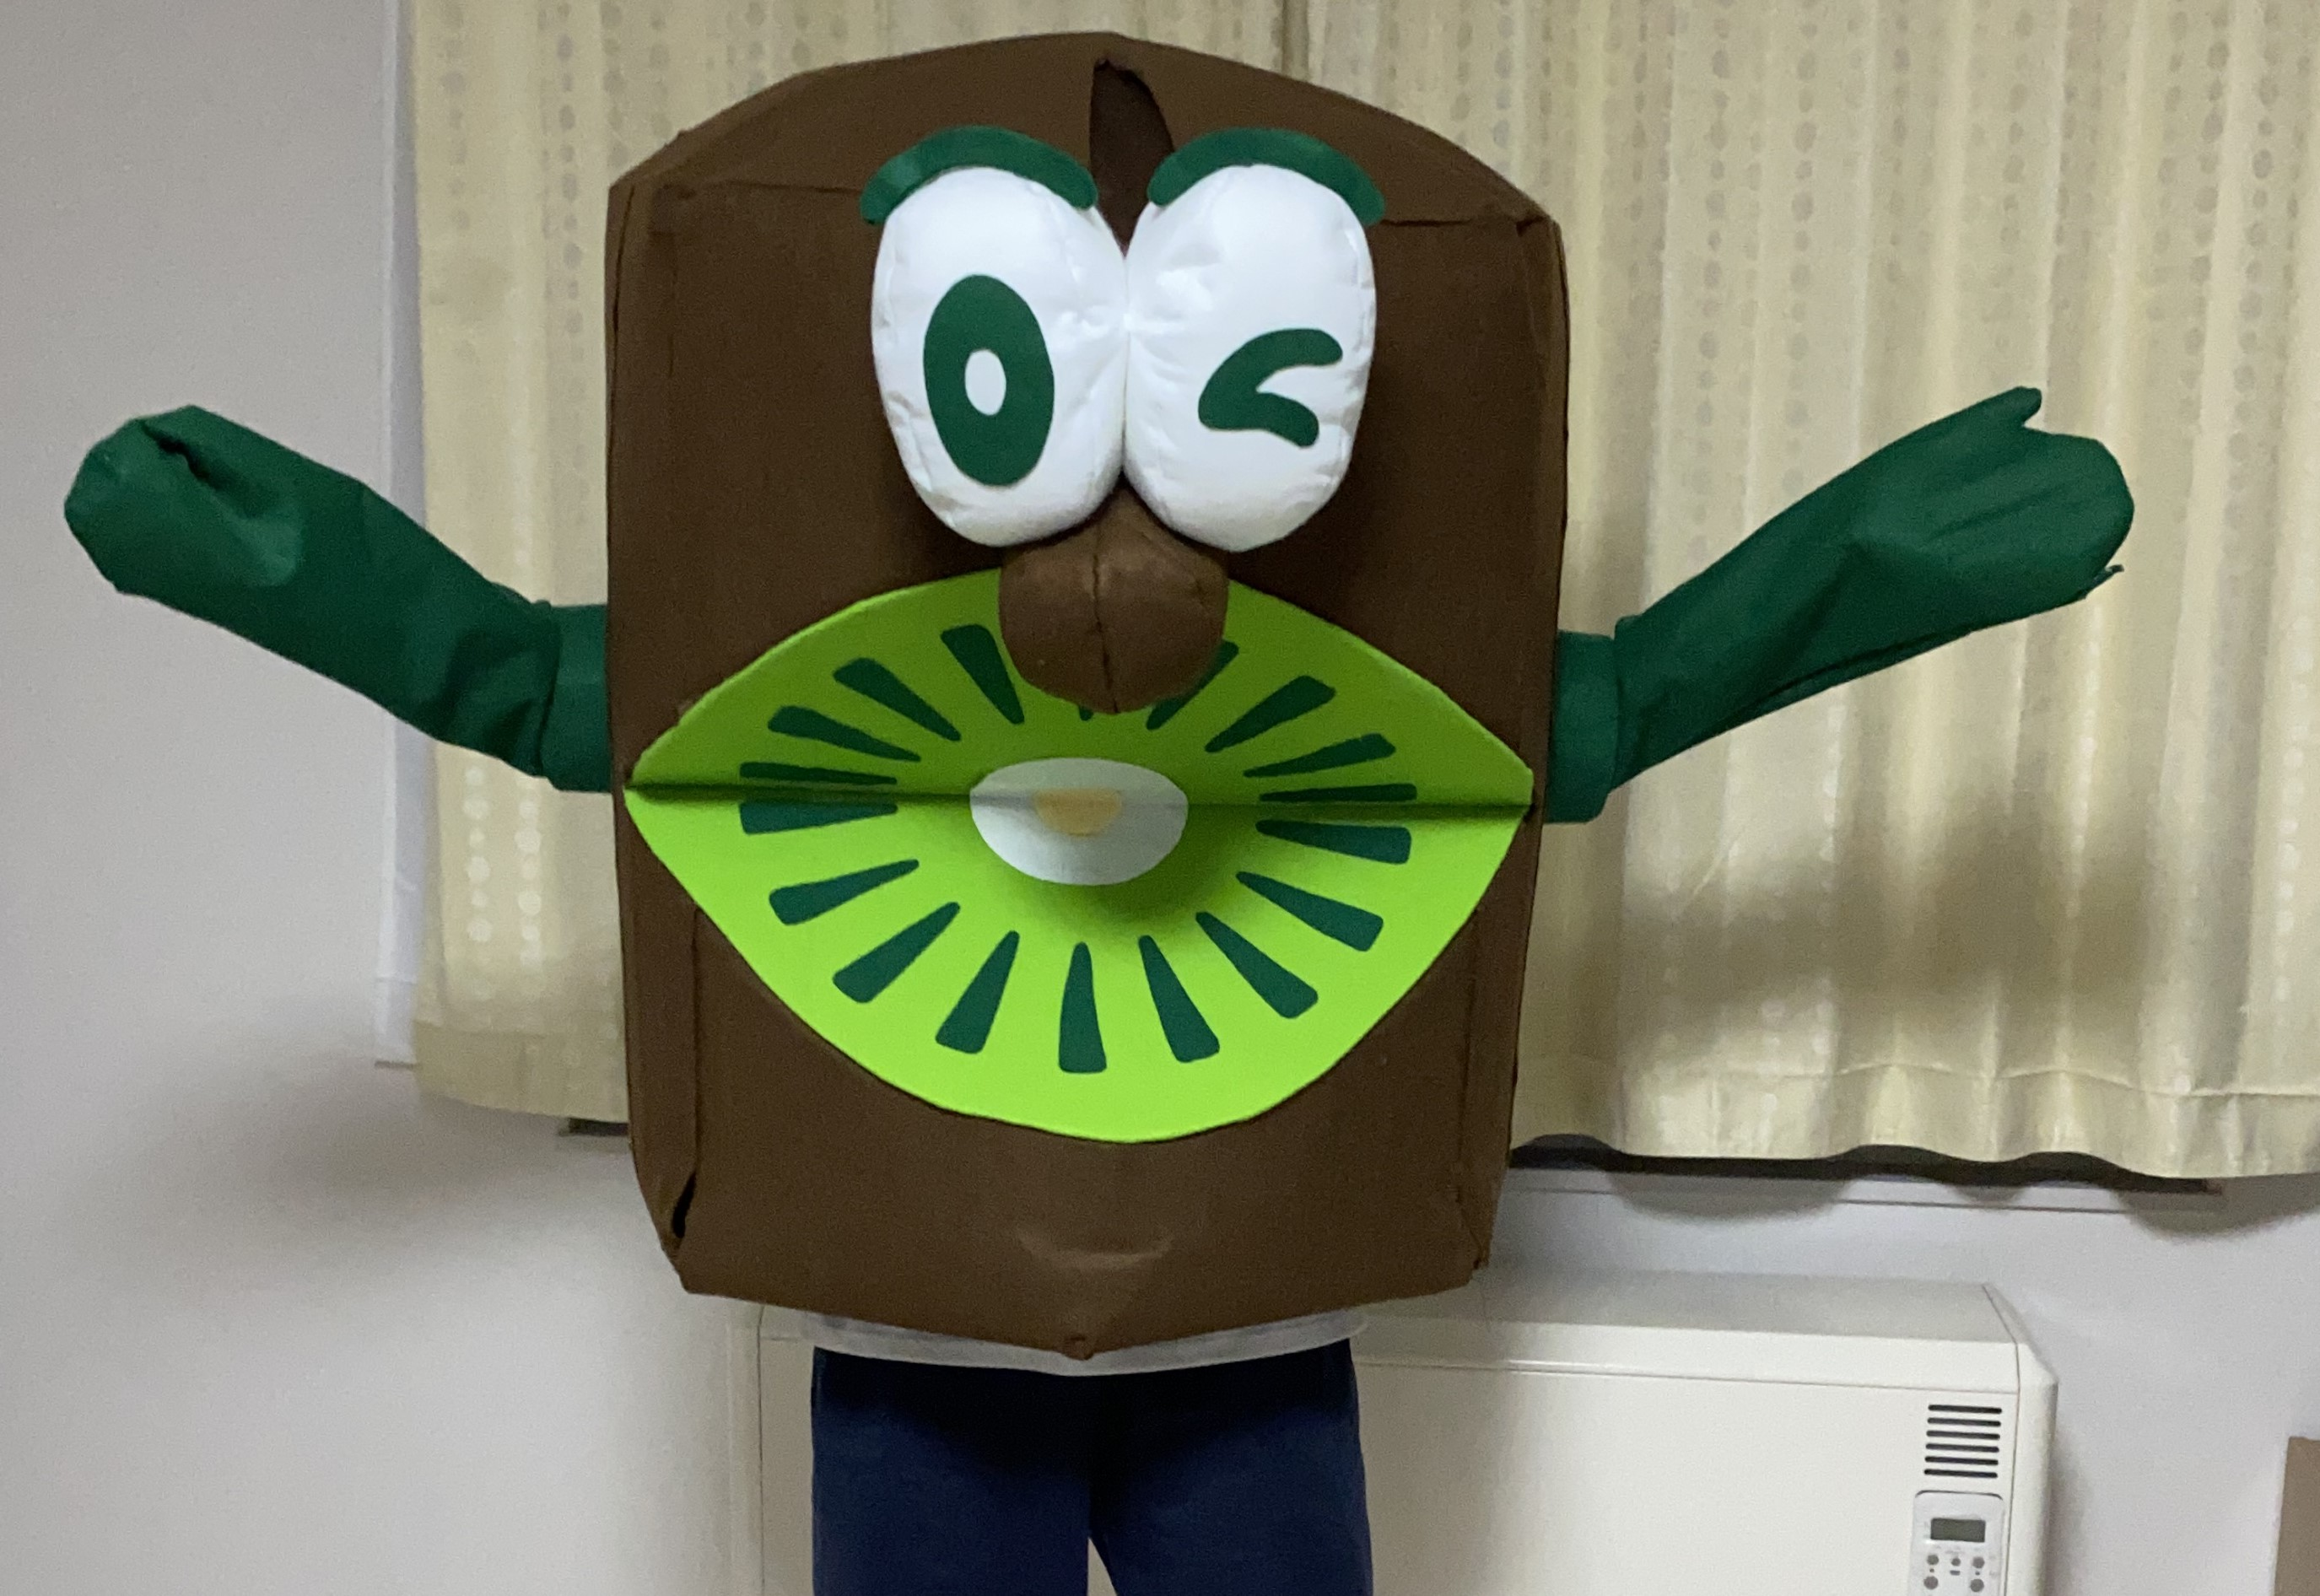
\includegraphics[width=0.8\hsize]{image/1/1.1.jpg}
        \caption{オリジナルキウイ}\label{fig:orikiui}
    \end{center}
    \vspace{0mm}
\end{figure}

\newpage

\begin{figure}[H]
    \vspace{0mm}
    \begin{center}
        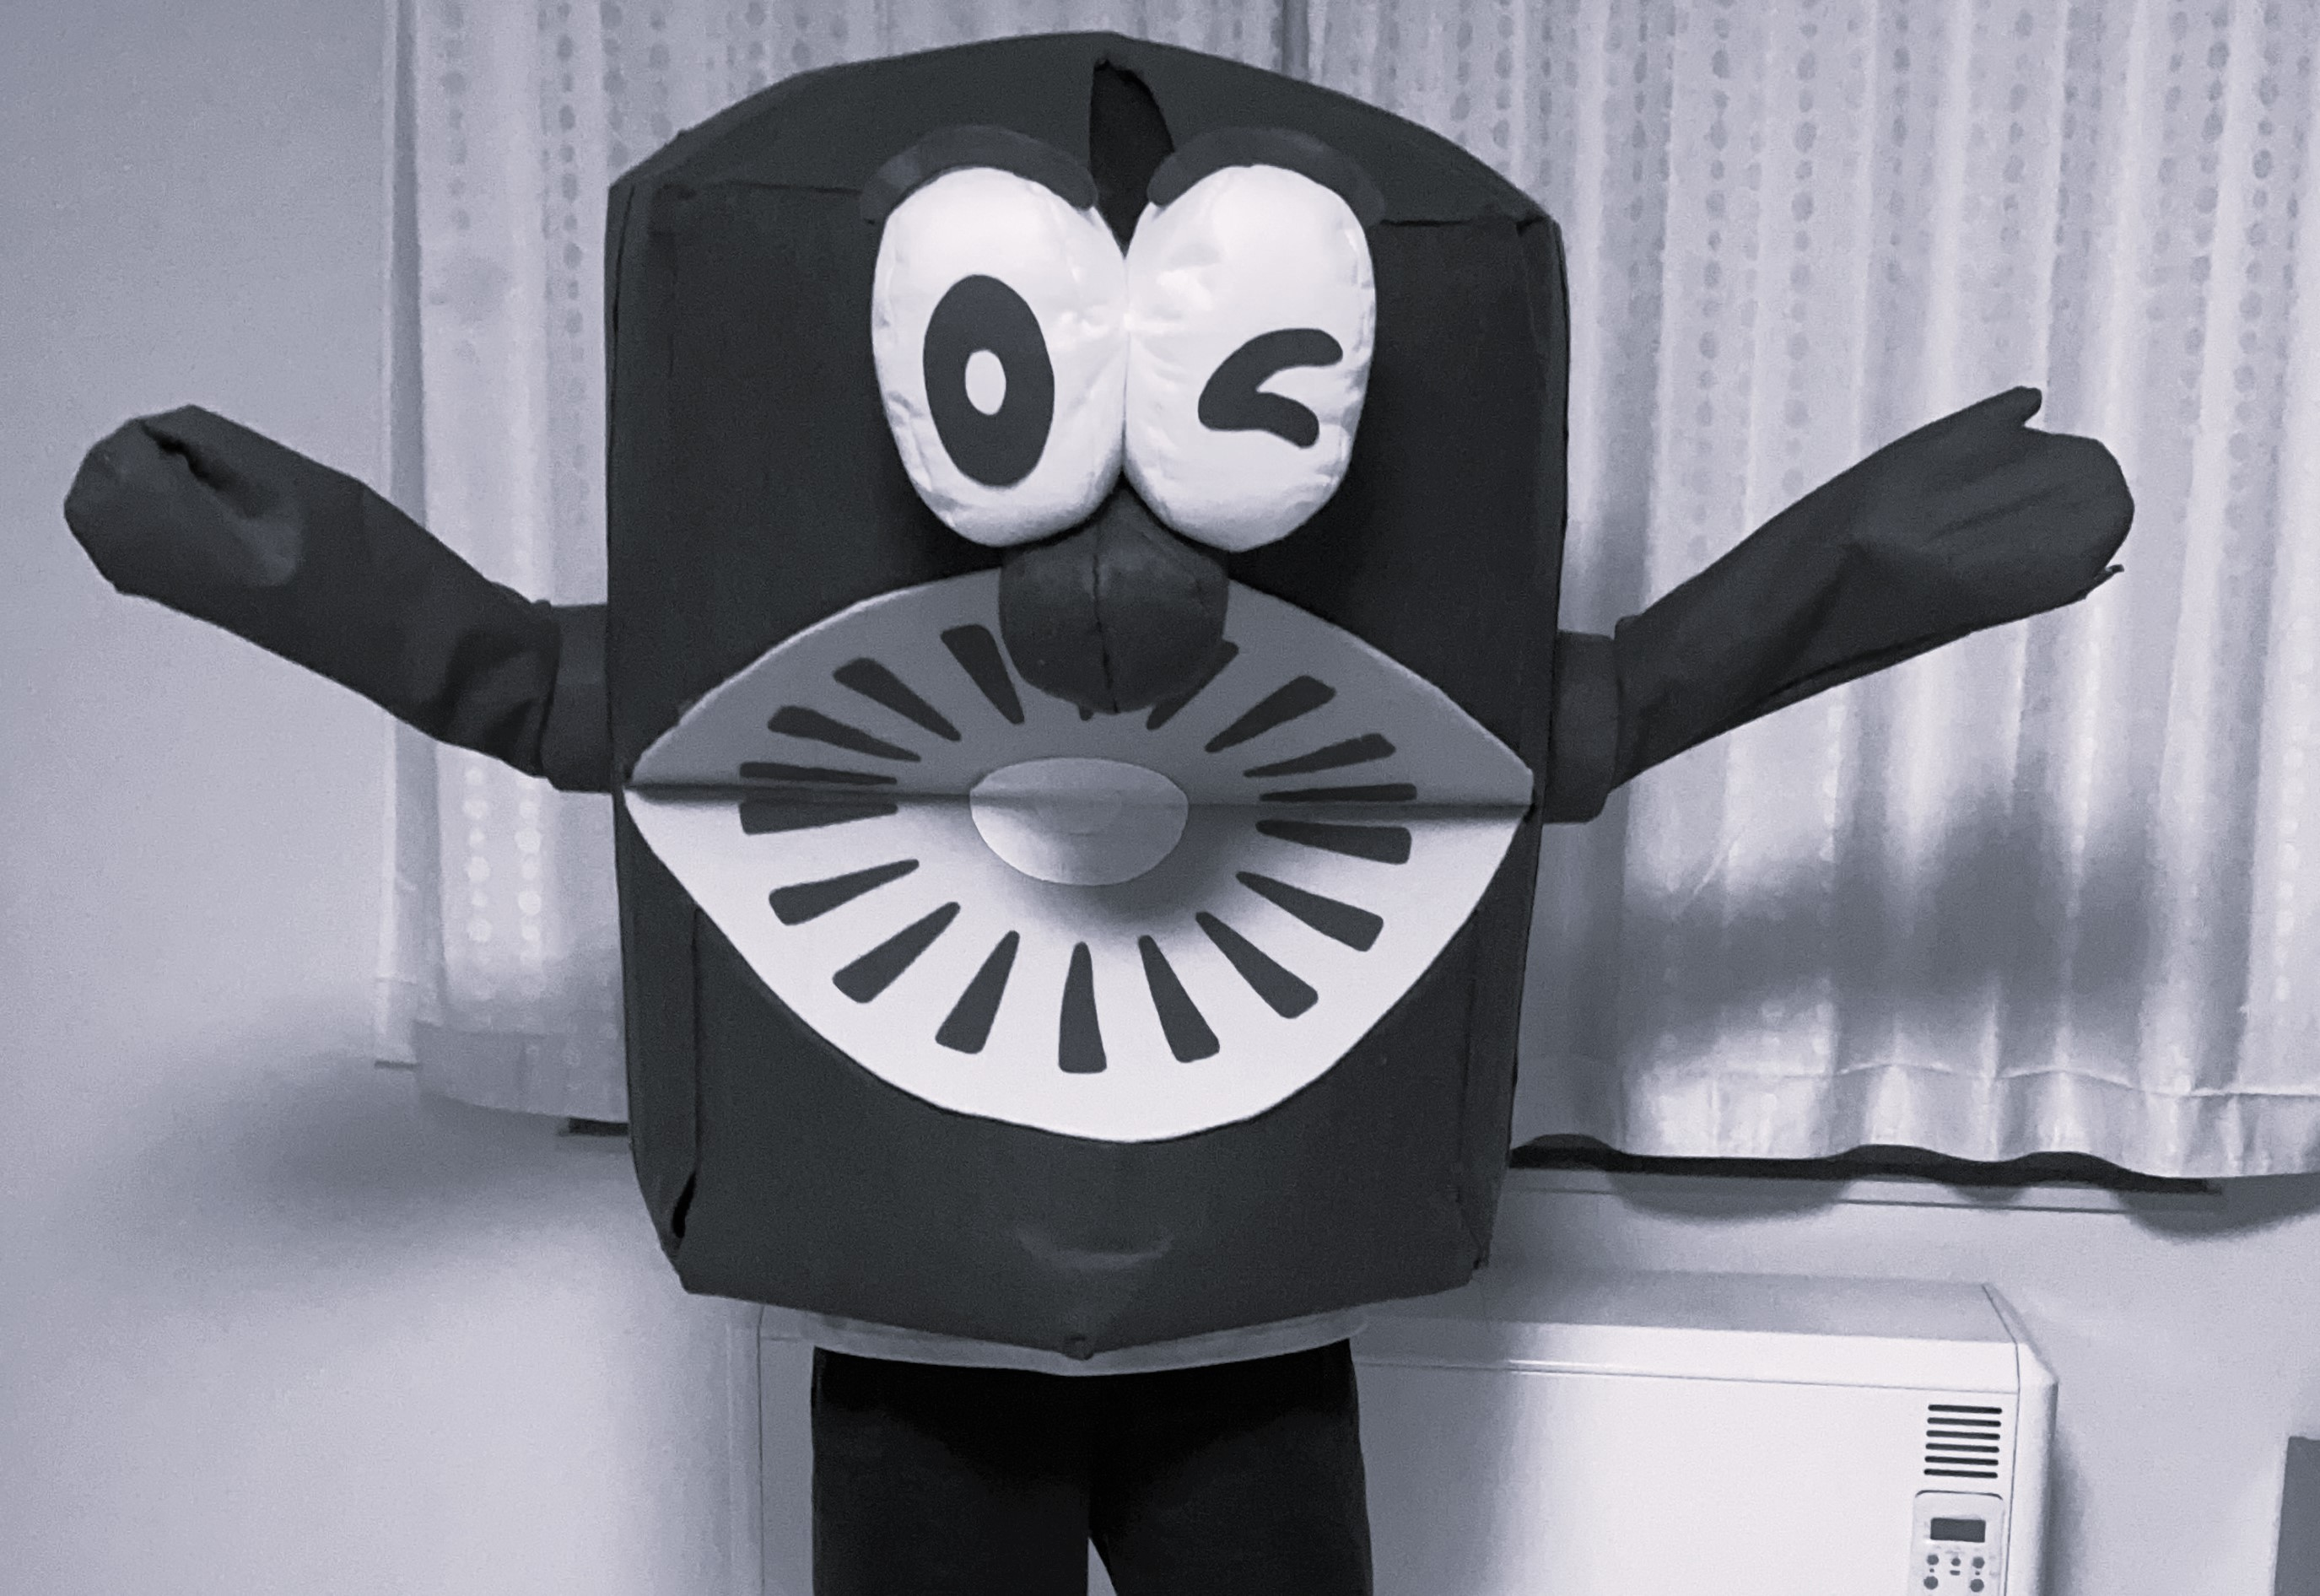
\includegraphics[width=0.8\hsize]{image/1/1.2.jpg}
        \caption{モノクロキウイ}\label{fig:monokiui}
    \end{center}
    \vspace{0mm}
\end{figure}

各コマンドの設定について説明する。

\begin{enumerate}
    \item \textbackslash begin\{figure\}[H]
    
        [H]は、"Here" を意味し、その場所に図を配置するように指示します。
        他のオプションもありますが、基本これでいいでしょう。

    \item \textbackslash vspace\{0mm\}
    
        画像の上下にスペースを入れます。基本的には0でいいでしょう。

    \item \textbackslash includegraphics[width=0.8\textbackslash hsize]\{image/1/1.1.jpg\}
    
        [width=0.8\textbackslash hsize]では、画像の幅を指定しています。
        もし、[width=1\textbackslash hsize]であれば、行の幅いっぱいに画像を拡大することを意味します。
        通常、画像の拡大率を1よりも小さくすることが一般的です。
        0.8や0.9などを試して、文章のレイアウトを保ちましょう。
        \{image/1/1.1.jpg\}では、表示する画像のパスを書きます。
        画像の数は多くなると管理が大変なので、章ごとに分けることをおすすめします。
        このテンプレートでは、"image">"章番号">"章番号.番目"というフォルダ構成になっています。
    
    \item \textbackslash caption\{オリジナルキウイ\}\textbackslash label\{fig:orikiui\}

        \textbackslash caption\{オリジナルキウイ\}で図名を付けます。
        \textbackslash label\{fig:orikiui\}では、文中で図番号を参照するときに使うラベルの設定です。
        短い言葉や略語を使用し、それぞれ意味のある名前にすることが重要です。
    
\end{enumerate}

\newpage

\subsection{表の出力}

以下に、表を出力する書き方を示す。

\begin{table}[H] % そのままコピーすると、レイアウトがひどいので"H"のみ追加
    \begin{tabular}{cccc}
    \hline
    品種名         & 果肉の色 & 早晩性 & 収穫時期の目安    \\ \hline
    香緑          & 緑色   & 晩性  & 10月下旬      \\
    ヘイワード       & 緑色   & 晩性  & 11月上旬~中旬   \\
    さぬきゴールド     & 黄色   & 早性  & 10月中旬      \\
    センセーションアップル & 黄色   & 早性  & 10月中旬~下旬   \\
    ゴールデンキング    & 黄色   & 早性  & 10月下旬      \\
    ジャンボイエロー    & 黄色   & 早性  & 11月上旬      \\
    レインボーレッド    & 赤色   & 早性  & 9月下旬~10月下旬 \\ \hline
    \end{tabular}
\end{table}

\begin{table}[H]
    \caption{キウイの収穫時期}\label{tab:zikikiui}
	\vspace{-5mm}
	\begin{center}
        \begin{tabular}{cccc}
        \hline
        品種名         & 果肉の色 & 早晩性 & 収穫時期の目安    \\ \hline
        香緑          & 緑色   & 晩性  & 10月下旬      \\
        ヘイワード       & 緑色   & 晩性  & 11月上旬~中旬   \\
        さぬきゴールド     & 黄色   & 早性  & 10月中旬      \\
        センセーションアップル & 黄色   & 早性  & 10月中旬~下旬   \\
        ゴールデンキング    & 黄色   & 早性  & 10月下旬      \\
        ジャンボイエロー    & 黄色   & 早性  & 11月上旬      \\
        レインボーレッド    & 赤色   & 早性  & 9月下旬~10月下旬 \\ \hline
        \end{tabular}
    \end{center}
\end{table}

表を作成するには、Tables Genratorという表作成ブラウザページを使うと楽だと思います。
Excelで作った表を画像として保存し、出力すると画質が荒くなるのでやめましょう。
Tables Genratorは基本Excelのような使い方でできるので問題ないと思います。
ただし、Excelの劣化版だと思ってください。我慢しましょう。
Tables Generatorを使って作成したtex文章をそのままコピーしたのが上の表です。
このままだとレイアウトが正しくないので、
下の表のように\textbackslash caption\{キウイの収穫時期\}\textbackslash label\{tab:zikikiui\}と\textbackslash vspace\{-5mm\}、
\textbackslash begin\{center\}を加えましょう。

\newpage

\section{図、表、参考文献の文中での参照}

ここでは図や表、参考文献を文中で参照する方法について説明します。
文中で、図や表、参考文献を示す場合は、以下のように書きましょう。
この書き方をすることにより、図表参考文献を後々追加しても、文章の図表参考文献番号が自動で変わるので手間が省けます。

\begin{enumerate}
    \item 図の参照
    
        新鮮なキウイを図\ref{fig:orikiui}に示す。
        100年後のキウイを図\ref{fig:monokiui}に示す。
    
    \item 表の参照
    
        キウイの収穫時期について表\ref{tab:zikikiui}に示す。
    
    \item 参考文献の参照

        表を作成するには、Tables Genratorという表作成ブラウザページを使うと楽だと思います\cite{TablesGenerator}。

\end{enumerate}

\section{箇条書き}

ここでは、箇条書きの書き方について説明する。
箇条書きでは、[enumitem]パッケージを使用して、\textbackslash begin\{enumerate\}[...] の中で番号の設定を行いましょう。
以下に、箇条書きの例を示す。

\begin{enumerate}[label=(\arabic*)] % [label=\Alph*],[label=\roman*],[label=\arabic*.],[label=\textbullet]
        \item グリーン

        \begin{enumerate}[label=\textbullet]
            \item 性格:まじめで、正義感が強く、しっかり者
            \item 自慢の栄養素:不足しがちな食物繊維が補える
            \item 特技:他の果物と仲良くすること(スムージー)
            \item 趣味:お惣菜コーナーまでの散歩
            \item チャームポイント:ワイルドな柔毛
            \item 座右の銘:蒔かぬ種は生えぬ
        \end{enumerate}

        \item ゴールド
        \item レッド
        \item キウイブラザーズ
\end{enumerate}
  %% 本文1
\chapter{数式・特殊文字}
\vspace{20mm}\hrulefill\\\vspace{20mm}

この章では、数式・特殊文字の書き方について、記載する。
前章でもお伝えしたが、ここに記載しているのはあくまでも最低限です。
詳しくTexについて学びたい方は、Googleで"謎肉 スースキス カップラーメン"などで検索して、♪勝手に スースキス スキスしてください。

\newpage

\section{数式}
LaTeXで数式を書くためには、いくつかの方法があります。
以下に、基本的な数式の書き方を示す。
\begin{enumerate}
	\item インライン数式
	
		インライン数式は、テキスト内に数式を埋め込む場合に使用する。
		数式を $ ... $で挟んで使います。
		
		ex.これはインライン数式 $E=mc^2$ です。

	\item ディスプレイ数式
	
		ディスプレイ数式は、独立した行に数式を表示する場合に使用されます。
		'equation'環境を使用します。
		
		ex.これはディスプレイ数式です:
		\begin{equation}
			\int_{0}^{\pi} \sin(x) \, dx = 2
		\end{equation}

		\begin{eqnarray}
			E_0 = {K}\cdot{I_0}\cdot{R_L}\ /\ {n}\  [\ \mathrm{V_{rms}}\ ]
		\end{eqnarray}

\end{enumerate}

\section{特殊文字}
Latexにはたくさんの特殊文字があります。
全部書ききれるわけがないので、適当にリストアップしたものを示します。
その他、コードを忘れた場合は、VScode左バーにある"TEX">"SNIPET VIEW"から選択するのもいいだろう。

\begin{enumerate}
	\item 数学記号と演算子
	
	$\alpha, \beta, \gamma, \theta, \pi, \sqrt{x}, \frac{1}{2}, \sum_{i=1}^{n} x_i, \int_{a}^{b} f(x) \, dx$

	\item 上付き文字と下付き文字

	$x^2, a_{ij}, e^{i\theta}, \lim_{x \to \infty}$

	\item 分数
	
	$\frac{a}{b}, \frac{\sqrt{2}}{2}$

	\item 行列
	
	$\begin{bmatrix}
		1 & 2 \\
		3 & 4
	\end{bmatrix}$

\end{enumerate}  %% 本文2
\chapter{参考文献の書き方}
\vspace{20mm}\hrulefill\\\vspace{20mm}

この章では、参考文献の書き方について、記載する。
前章、前前章でもお伝えしたが、ここに記載しているのはあくまでも最低限です。
詳しくTexについて学びたい方は、Googleで"3人そろってにしたん"などで検索して、♪勝手に、にしたんたんたんたーんしてください。

\newpage

\section{参考文献}

このテンプレートでは、Bibtexを使用して参考文献の作成を行っています。
参考文献のデータベースを.bibという拡張子のファイルに書き込んでいきます。
書き方としては、@Articleや@Bookなどから\{\}の中身までが文献1つにあたる。
@の次が文献の種別を表すもので、表1のような種類がある。

\begin{table}[H]
	\caption{BibTeXの文献種別と一言説明}\label{tab:bibtex-entry-types}
	\vspace{-5mm}
	\begin{center}
		\begin{tabular}{cc}
		\hline
	  	\normalfont\textbf{文献種別} & \normalfont\textbf{一言説明} \\\hline
	  	article & 学術論文(雑誌論文や雑誌記事) \\
	  	book & 単行本 \\
		online & オンライン資料 \\
	  	booklet & 書籍全体ではなく、印刷物全体に対する参照 \\
	  	inbook & 本の中の一部(章や節など) \\
	  	incollection & 編集された本や論文集の中の一部 \\
	  	inproceedings & 学会論文集や会議録の中の一部 \\
	  	manual & マニュアルや技術的なドキュメント \\
	  	mastersthesis & 修士論文 \\
	  	misc & 他のどの種別にも合致しないもの \\
	  	phdthesis & 博士論文 \\
	  	proceedings & 学会論文集や会議録全体 \\
	  	techreport & 研究所や大学のテクニカルレポート \\
	  	unpublished & 公式に発表されていない文献 \\\hline
		\end{tabular}
	\end{center}
\end{table}  %% 本文3
% 章数に応じて適宜追加

% 参考文献
\addcontentsline{toc}{chapter}{\bibname} % 目次に"参考文献"を表示
\nocite{*} % 文書内で引用していない文献を全て引用
\bibliographystyle{jplain} % 参考文献をアルファベット順で出力する
\bibliography{demobib}  %% 参考文献(拡張子.bibを除いたファイル名)

% 謝辞
\begin{acknowledgment}

kudo研の皆さん、texの環境構築お疲れさまでした。そして、論文の執筆ご苦労様でした。
相当大変だったでしょう。
しかし、休んでいる暇はありません。
論文要旨でも言ったように、この一年間やったことを " 後輩につなぐ " 資料の作成をぜひお願いします。

"めっちゃ結果出せた!"、"うまく進まなかったなぁ"、"さぼりすぎた・・・"

いろんな人がいるでしょう。悪い成果も立派な研究の資料です。
データ、制作物、説明書、文献、後悔の念、すべて文章として残してから卒業してくれることを祈っています。

\end{acknowledgment} %%

% 付録
\appendix
\renewcommand{\chaptermark}[1]{\markboth{付録\ \thechapter\ ~#1}{}}
\setcounter{page}{1}
\pagenumbering{Roman}
\chapter{}\label{chap:appendixA}
\vspace{20mm}\hrulefill\\\vspace{20mm}

\section{制作したプログラム}

\begin{lstlisting}[caption=greeting.py,label=greeting.py]
    # ユーザーに名前を尋ねて挨拶するプログラム

    # ユーザーに名前を尋ねる
    name = input("あなたの名前は何ですか? ")
    
    # 名前を使って挨拶する
    print("こんにちは、" + name + "さん!")
\end{lstlisting}

\section{面白いプログラム}

\begin{lstlisting}[caption=tell\_joke.py,label=joke.py]
    import random

    def tell_joke():
        jokes = [
            "なぜプログラマーはコーヒーを飲むのですか?因数分解です。",
            "なぜPythonはクールですか?冷静なエンジニアが作ったから。",
            "なぜコンピュータは冷たい飲み物が好きですか?氷が付いてくるから。",
            "なぜサーバーはいいことを言わないのですか?お世辞を言うとサービスがダウンします。",
            "なぜプログラマーは山登りが好きですか?山がピークだから。",
        ]
    
        joke = random.choice(jokes)
        print("ジョーク: " + joke)
    
    # ジョークを表示
    tell_joke()
    

\end{lstlisting}
 %% 付録A
\chapter{}\label{chap:appendixB}
\vspace{20mm}\hrulefill\\\vspace{20mm}

\section{キウイと鳥のキウイ、そしてきゅうりの違いについて}

キウイ、鳥のキウイ、そしてきゅうりは、それぞれ異なる生物でありながら偶然にも名前が似ています。
これらの存在は見た目や生態だけでなく、食品としての利用法や文化的背景においても多様性を持っています。

\subsection{1. キウイ(果物)}

キウイは、茶色い繊維状の外皮と緑色の果肉を持つ独特の形状をした果物です。
もともとは中国原産で、ニュージーランドで栽培が成功しました。
ビタミンCや食物繊維が豊富で、爽やかで甘酸っぱい味わいが特徴です。
生食はもちろん、デザートやサラダの材料としても広く愛されています。

\subsection{2. 鳥のキウイ}

一方で、鳥のキウイは、キウイの名前を冠する夜行性の鳥です。
小さな目、翼がなく、大きな卵を産む特異な外見を持ちます。
ニュージーランド原産の鳥で、絶滅の危機に瀕しています。
長いくちばしや茶色の羽毛が特徴的で、保護が喫緊の課題となっています。

\subsection{3. きゅうり}

きゅうりは、野菜として広く知られ、世界中で栽培・消費されています。
爽やかな風味があり、サラダやピクルス、スムージーなど多岐にわたる料理に利用されます。
キウイと同じく名前に"キュ"が含まれていますが、全く異なる分類の食材です。
その形状や用途は、果物のキウイや鳥のキウイとはまったく異なります。
kudo先生が嫌いな食べ物です。

これらの「キウイ」は、名前の類似性にもかかわらず、それぞれが自然界で異なる役割を果たしています。
生活の中でこれらの違いを理解することは、多様性を尊重し、異なる存在の美しさを感じる手助けとなります。
 %% 付録B
% 付録数に応じて適宜追加

\end{document}
